\chapter{Фотопереключатели на основе (гет)арилстильбенов и краун-эфиров. ESIPT люминесценция (обзор литературы)} \label{chapt1}

	Среди большого разнообразия различных органических фотопереключателей особую роль играют фотопереключатели на стильбенах и их гетероциклических аналогах. Стильбены обладают как хорошей люминесценцией \cite{Krasovitsky_Bolotin}, так и способностью к высокоэффективному быстрому фотопереключению. Стильбены отличаются относительной простотой в получении \cite{Wood1941} и широкой возможностью для модификации функциональными заместителями и гетероциклическими фрагментами, что позволяет создавать структуры со сложным фотофизическим и фотохимическим поведением. \cite{Waldeck_D_H1991_Stilbenes} 
	
	Гетероциклические аналоги стильбенов позволяют улучшить люминесцентные свойства за счёт создания сопряжённой донорно-акцепторной пары. Наличие акцепторного азинового (азинонового) ядра в молекулах благодаря вкладу \textit{n},$\pi$*-состояния может оказывать заметное влияние на фотохимическое и фотофизическое поведение люминофоров. \cite{Lower1966} Азотсодержащие гетероциклические фрагменты, такие как пиримидин, хиназолин, хиноксилин и другие, зарекомендовали себя как хорошие акцепторные заместители, обладающие как собственной люминесценцией \cite{Krasovitsky_Bolotin}, так и работающие в паре с арильными донорами.
	
	Краун-содержащие (гет)арилстильбены хорошо представлены в литературе \cite{Gromov_2006_Crowns_in_Stilbenes}. В основном, краун или бензокраунсодержащий фрагмент является частью стильбена. 

	\section{Синтез, фотофизические и фотохимические свойства гетероциклических аналогов стильбенов}\label{sect1_1}
	
		\subsection{Синтез}
	
			Одним из наиболее известных способов получения карбоциклических стильбенов является восстановление бензоила или бензила амальгированным цинком в кислой среде. \cite{Krasovitsky_Bolotin} 
			
			\begin{scheme}
				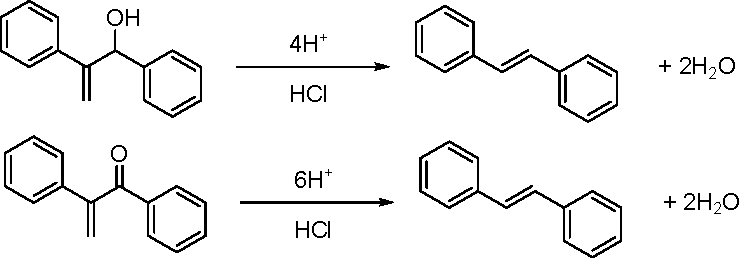
\includegraphics{Dissertation/images/part1/Stylbenes}	
			\end{scheme}
			
			Также часто используется реакция конденсации альдегида на толуоле благодаря подвижности водородов метильной группы. \cite{Wood1941} Разнообразие исходных реагентов позволяют получать различные функционализированные стильбены. 
			
			\begin{scheme}
				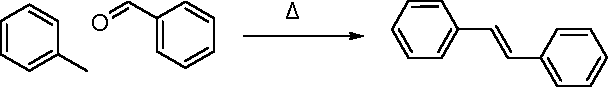
\includegraphics{Dissertation/images/part1/Stylbenes2}	
			\end{scheme}
		
			Кроме того, возможно получение диарилэтенов при помощи методов, основанных на использовании диазасоединений.\cite{Krasovitsky_Bolotin} Например, можно получить стильбен, 1,4-дистирилбензол и их аналоги с ароматическими радикалами конденсацией арилдиазонийхлоридов   со стиролом или коричной кислотой. Таким образом были получены 4-метил, 4-хлор, 4-гидрокси, 4-метокси, 4-этоксистильбены. \cite{Scintilators} Другим методом, основанном на азотсодержащих соединениях является термическое разложение азинов. \cite{Malkes1962_5} Таким методом можно получать несимметричные стильбены. Наиболее эффективно процесс протекает при 300\textdegree{}С. Тем не менее, такой способ имеет недостатки. Так авторы отмечают образование в виде побочных продуктов реакции бензонитрила, аммиака, бензальамина и 2,4,5-трифенилбензимидазола. При разложении 1-(1-нафталь)-2-(2-нафталь)азина наблюдалось образование 1,2-ди-(2-нафтил)этилена, а при разложении 1-(1-нафталь)-2-(4-бифенилаль)азина -- 1,2-ди-(4-бифенилил)этилен. Для получения диарилэтиленов, содержащих 1-нафтильные радикалы, реакцию проводили в присутствии порошка меди.\cite{Malkes1962_1}
			
			\begin{scheme}
				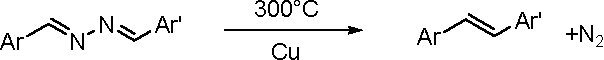
\includegraphics{Dissertation/images/part1/Stylbenes3}	
			\end{scheme}
		
			Несимметричные 1-фенил-2-нафтилэтены получают декарбоксилированием арилакриловых кислот нагреванием их с медной бронзой в хинолине. Подобные методы также применяются при образовании дистирилбензолов.
			
			Огромный интерес представляют собой гетероциклические аналоги стильбенов. \cite{Taek1987, Liang2003, Lipunova2011} основной способ синтеза подобных соединений -- это конденсация альдегида на метильной группе гетероциклического реагента в уксусной кислоте. \cite{Nosova2011, Lipunova2011, Ouyang2009a, Wang2009, Liang2003, Yim2008, Cazaux1993} Такой способ позволяет контролировать расположение гетероатомов в кольце, расположение заместителей в карбо- или гетероцикле. 
		
		
		\subsection{Фотофизические и фотохимические свойства стильбенов и их гетероциклических аналогов}
		
			Текст первой главы
			
			\begin{scheme}
				%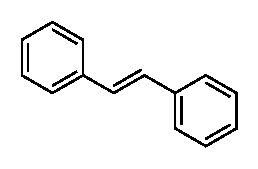
\includegraphics{Dissertation/images/part1/Stilbene}
			\end{scheme}
			
			
			
			
			